\section{Results}\label{sec:results}
%Results
%Show effect of colorspaces, blur, annealed mean
%Compare results of architecture (images, error plot, feature maps)
	
In section \ref{sec:method} all the different techniques and methods used resulted in multiple experiments. This sections shows the different results of each experiment, setting the foundation for the discussion.

\subsection{Colorspace}
To asses the effect of different colorspaces, a comparison is made between CIELab and YCbCr. The compact network architecture is trained on the landscape set for both the YCbCr and CIELab color space, for a total of 20 epochs. The result is shown in figure \ref{fig:YCbCr_vs_CIELab}. The CIELab colorspace has more saturated colors than the YCbCr output. Similar results were found by Iizuka et al. \cite{IizukaSIGGRAPH2016}.

\begin{figure}
	\begin{minipage}{.5\textwidth}
		
		\centering
		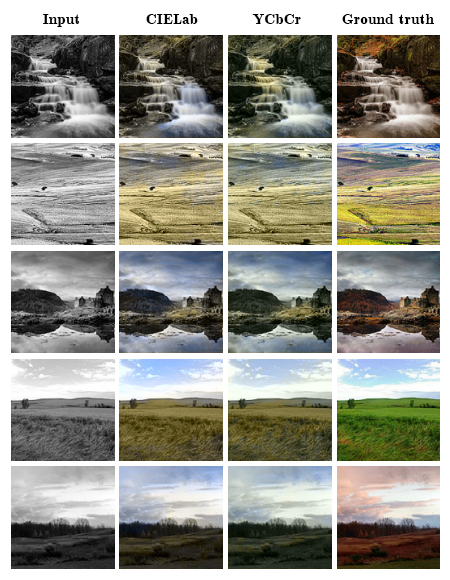
\includegraphics[width=0.78\textwidth]{YCbCr_vs_CIELab}
		\caption{YCbCr vs CIELab}
		\label{fig:YCbCr_vs_CIELab}
		
	\end{minipage}
	\begin{minipage}{0.5\textwidth}
			\centering
			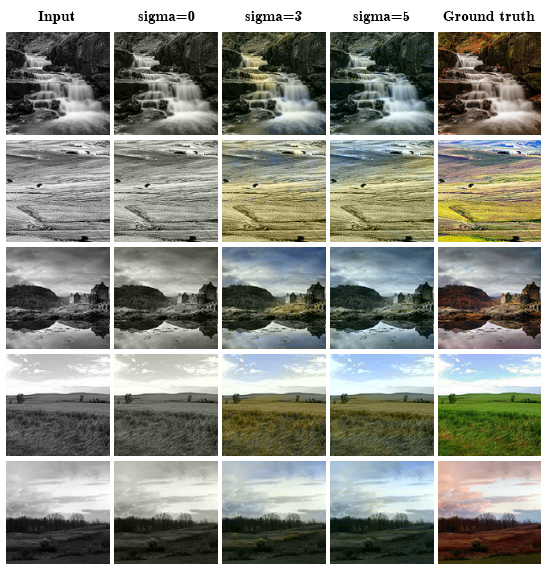
\includegraphics[width=0.95\textwidth]{blur}
			\caption{Blur}
			\label{fig:blur}
	\end{minipage}
\end{figure}

\subsection{Gaussian blur}
The comparison between different Gaussian blur kernel size is seen in figure \ref{fig:blur}. The comparison was done with the compact network, trained on the landscape dataset. Note that the kernel size only comes into play during training, since the target output layer is blurred the target less noisy. For no blur, the network converged to an almost grayscale image. For $\sigma = 3$ and $\sigma = 5$ the network did learn to colorize images. With $\sigma = 5$ the images look like they have a blue overlay.

\subsection{Network output}
In this section the colorization result of the different networks are shown, by propagating an image through the trained networks. These results are shown in figure \ref{fig:results}. Note that the annealed mean temperature is set to $0.4$. The optimal setting for the temperature can vary for each network, however keeping this into account sound conclusions can still be made. The compact network output has a lower saturation compared to the other networks. {\color{red} Hier nog de andere verschillen uit leggen zonder interpretatie te geven!}

\clearpage
\begin{figure}[h!]
	\centering
	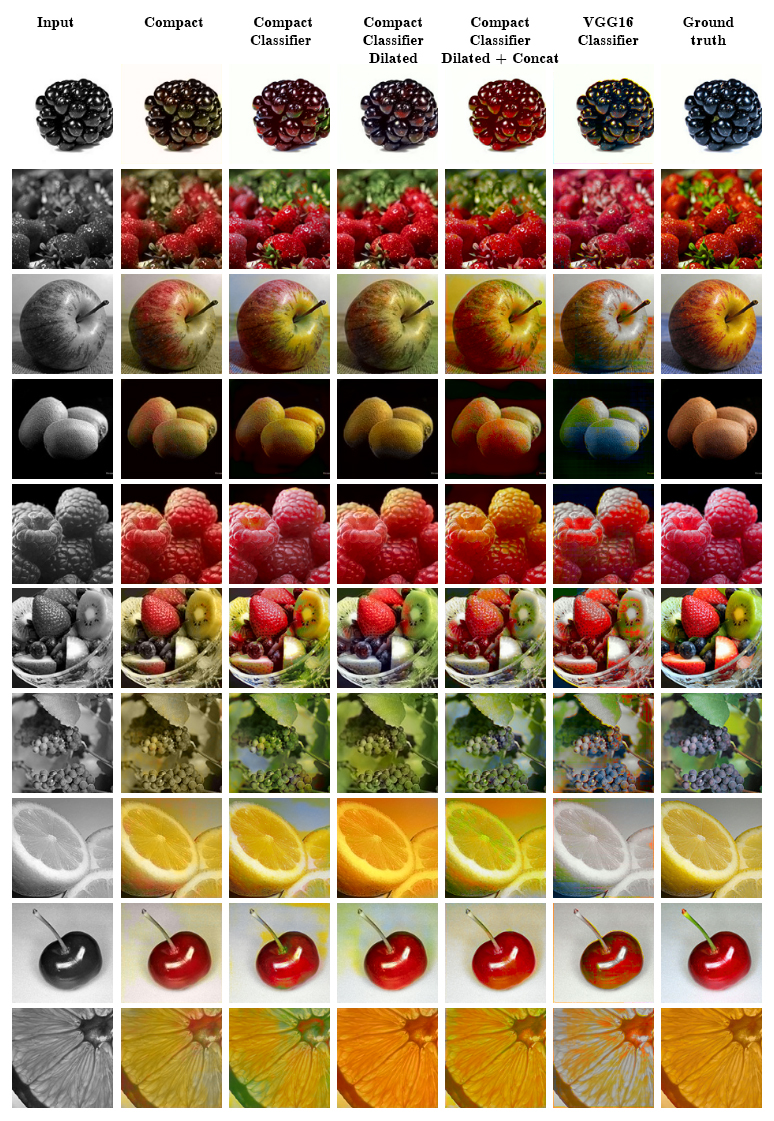
\includegraphics[width=0.9\textwidth]{set2}
	\caption{Results}
	\label{fig:results}
\end{figure}



